%%%%%%%%%%%%%%%%%%%%%%%%%%%%%%%%%%%%%%%%%%%%%%%%%%%%%%%%%%%%%%%%%%%%%%%%%%%%%%
\documentclass[12pt,a4paper,titlepage,final]{article}
% cestina a fonty
\usepackage[czech]{babel}
\usepackage[utf8]{inputenc}
% obrazky
\usepackage[dvipdf]{graphicx}
% velikost stranky
\usepackage[top=3.5cm, left=2.5cm, text={17cm, 24cm}, ignorefoot]{geometry}
%% cislovani objektu
\usepackage{chngcntr}
\counterwithin{figure}{section}
%reference v toc
\usepackage[nottoc,numbib]{tocbibind}
% balicky pro odkazy
\usepackage{color}
\usepackage{url}
\usepackage{tabularx}
\usepackage[unicode,colorlinks,hyperindex,plainpages=false,pdftex,linktoc=all]{hyperref}
\definecolor{urlBlue}{rgb}{0.1,0,0.7}
\definecolor{citeGreen}{rgb}{0,0.5,0}
\definecolor{linkRed}{rgb}{0.8,0.1,0.1}
\definecolor{fileSteelBlue}{rgb}{0,0.2,0.4}
\hypersetup{
    linkcolor=linkRed,          % color of internal links
    citecolor=citeGreen,        % color of links to bibliography
    filecolor=fileSteelBlue,    % color of file links
    urlcolor=urlBlue            % color of external links
}

\begin{document}

%%%%%%%%%%%%%%%%%%%%%%%%%%%%%%%%%%%%%%%%%%%%%%%%%%%%%%%%%%%%%%%%%%%%%%%%%%%%%%
% titulní strana

\def\projname{Počítačové vidění}
\def\projsubname{Skládání snímků}

\begin{titlepage}

\begin{center}
  \begin{large}
    \bf{Fakulta Informačních Technologií} \\
    \vspace*{0.5cm}
    \bf{Vysoké Učení Technické v~Brně}
  \end{large}
\end{center}

\vfill

\begin{figure}[!h]
  \centering
  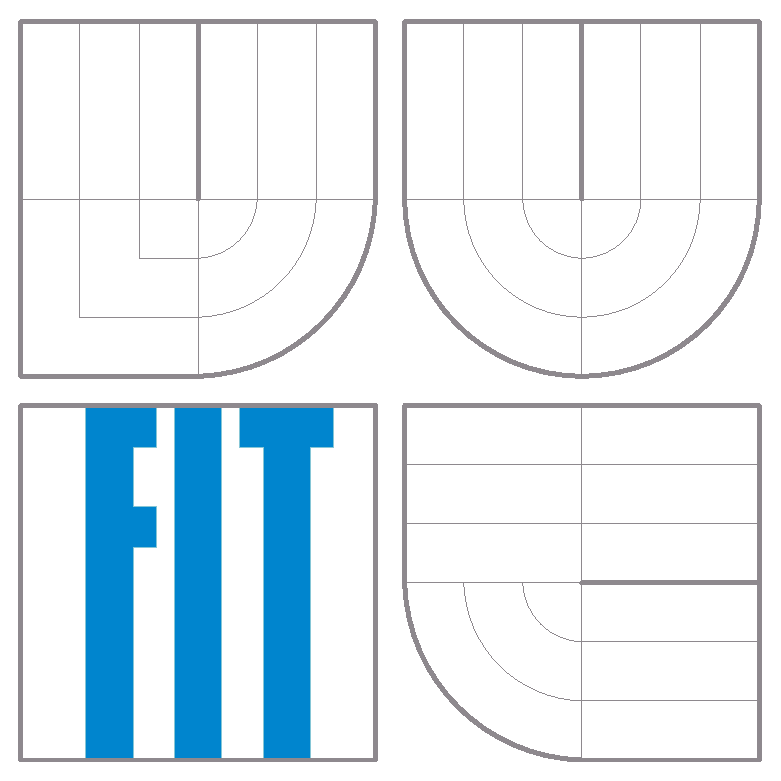
\includegraphics[height=5cm]{img/logo.eps}
\end{figure}

\vfill

\begin{center}
  \bigskip
  \begin{Huge}
    \bf{\projname}\\
  \end{Huge}

  \vspace*{1cm}

  \begin{Large}
    \bf{\projsubname}
  \end{Large}

  \vspace*{0.75cm}

  \begin{Large}
    \today
  \end{Large}
\end{center}

\vfill

\begin{large}
    \begin{tabularx}{\textwidth}{lXr}
      Ondřej Janošík & & xjanos12 \hspace{1.25cm} \\
      Vojtěch Kaisler & & xkaisl00 \hspace{1.25cm} \\
    \end{tabularx}
\end{large}

\end{titlepage}


%%%%%%%%%%%%%%%%%%%%%%%%%%%%%%%%%%%%%%%%%%%%%%%%%%%%%%%%%%%%%%%%%%%%%%%%%%%%%%
% obsah
\pagestyle{plain}
\pagenumbering{roman}
\setcounter{page}{1}
\tableofcontents

%%%%%%%%%%%%%%%%%%%%%%%%%%%%%%%%%%%%%%%%%%%%%%%%%%%%%%%%%%%%%%%%%%%%%%%%%%%%%%
% textova zprava
\newpage
\pagestyle{plain}
\pagenumbering{arabic}
\setcounter{page}{1}

%%%%%%%%%%%%%%%%%%%%%%%%%%%%%%%%%%%%%%%%%%%%%%%%%%%%%%%%%%%%%%%%%%%%%%%%%%%%%%
\section{Úvod}

Tato práce se zabývá automatickým spojováním obrázků.
Toho se často využívá při tvorbě panoramat a 360~stupňových pohledů.

\section{Teorie}

Při spojování obrázků je třeba nejdříve nalézt na obrázcích alespoň 4~páry
společných bodů. Tyto body je možné zadat manuálně, čímž je možné dosáhnout
vyšší přesnosti při výsledném spojování, nebo je můžeme získat algoritmicky.

Manuální zadávání však při velkém počtu snímků vyžaduje spoustu práce a příliš
velké výhody oproti algoritmickému vyhledávání nepřináší.
Algoritmické vyhledávání se skládá ze několika základních kroků a tím je nalezení
význačných bodů v obou obrázcích a nalezení odpovídajícího páru v sousedním
obrázku.

Z odpovídajících párů bodů je možné vypočítat transformaci, druhého obrazu vůči
prvnímu. Pokud aplikujeme zpětnou transformaci na druhý obraz, pak bude tento
obraz v ideálním případě pěkně navazovat na první obraz.
Tento postup je možné aplikovat pro více obrázků a vytvořit tak výsledné panorama.

\subsection{Hledání význačných bodů}

K nalezení význačných bodů v obraze slouží například metody SIFT a SURF. 
Metoda SURF (Speeded Up Robust Features) hledá význačné body a pro každý bod
vytváří deskriptor deskriptor jeho oblasti, který je invariantní vůči
zvětšení a rotaci.

\subsection{Nalezení podobných bodů}

Pro nalezení odpovídajích párů je potřeba, aby se obrázky dostatečně překrývaly.
Dále je vhodné, aby se právě v překrývající oblasti vyskytovalo co nejvíce význačných
bodů.

Určování odpovídajících bodů je založeno na knihovně FLANN (Fast Library for
Approximate Nearest Neighbors). Jedná se o knihovnu pro hledání přibližně
nejbližších sousedů ve vysoce dimensionálních prostorech.

\subsection{Výpočet transformace}

Algorimus pro nalezení podobných bodů může nalézt shody i v nepřekrývajících se
oblastech, je však jasné, že ne všechny význačné body se cházejí v překrývající
se oblasti a tudíž všechny body nemohou tvořit pár.

Pro určení těchto odpovídajích párů je použita metoda RANSAC. Jedná se o
nedeterministickou iterativní metodu, která dokáže vytvořit matematický model
z množiny dat, která obsahuje data, které do této množiny nepatří (tzv. outliers).

V našem případě vybere tato metoda vektory, které v množině dat převažují.
Tyto vektory pak odpovídají hledáným dvojicím bodů a je možné z nich vypočítat
potřebnou transformaci.

\subsection{Spojení obrázků}

Výsledné spojení je již relativně jednoduché. Stačí na obrázky aplikovat zpětné
transformace a skládat je do výsledného obrazu.
Ovšem při spojování většího počtu obrázku dochází u krajních obrázků ke značné
deformaci. V praxi se proto používá projekce na válec či kouli.
Dále mohou být viditelné přechody mezi obrázky. Klasický alfa blending
sice může tyto přechody zmírnit, ale na druhou stranu vytváří nepříjemné
artefakty. Vhodnější metodou je graph-cut, která vytvoří přechod v místě, kde
není tak viditelný (například na hranách objektů).

\section{Vyhodnocení}

Podařilo se nám vytvořit aplikaci, která nějak funguje a něco dělá.
Implementovali jsme projekci na kouli, která sama o sobě funguje, ale k lepším
výsledkům příliš nepřispívá. Dále jsme implementovali vyrovnání obrazu, aby 
výsledek vypadal trochu rozumně.

\section{Závěr}

Do slušného panoramatu by bylo třeba vynaložit ještě docela dost úsilí.

%%%%%%%%%%%%%%%%%%%%%%%%%%%%%%%%%%%%%%%%%%%%%%%%%%%%%%%%%%%%%%%%%%%%%%%%%%%%%%

%\bibliographystyle{czplain}
%\bibliography{zdroje}

%%%%%%%%%%%%%%%%%%%%%%%%%%%%%%%%%%%%%%%%%%%%%%%%%%%%%%%%%%%%%%%%%%%%%%%%%%%%%%
\end{document}
